\chapter{Środowisko badawcze: aplikacja Robot Shop, symulacja incydentów oraz uruchamianie epizodów}

\section{Aplikacja Robot Shop}
Podstawą środowiska badawczego jest aplikacja \textit{Robot Shop} -- demonstracyjny system e-commerce zbudowany w architekturze mikrousługowej. Aplikacja ta została wybrana ze względu na odzwierciedlenie rzeczywistych wzorców projektowych oraz wykorzystanie różnorodnych technologii składowych, co czyni ją reprezentatywnym modelem dla systemów produkcyjnych.

\begin{figure}[H]
  \centering
  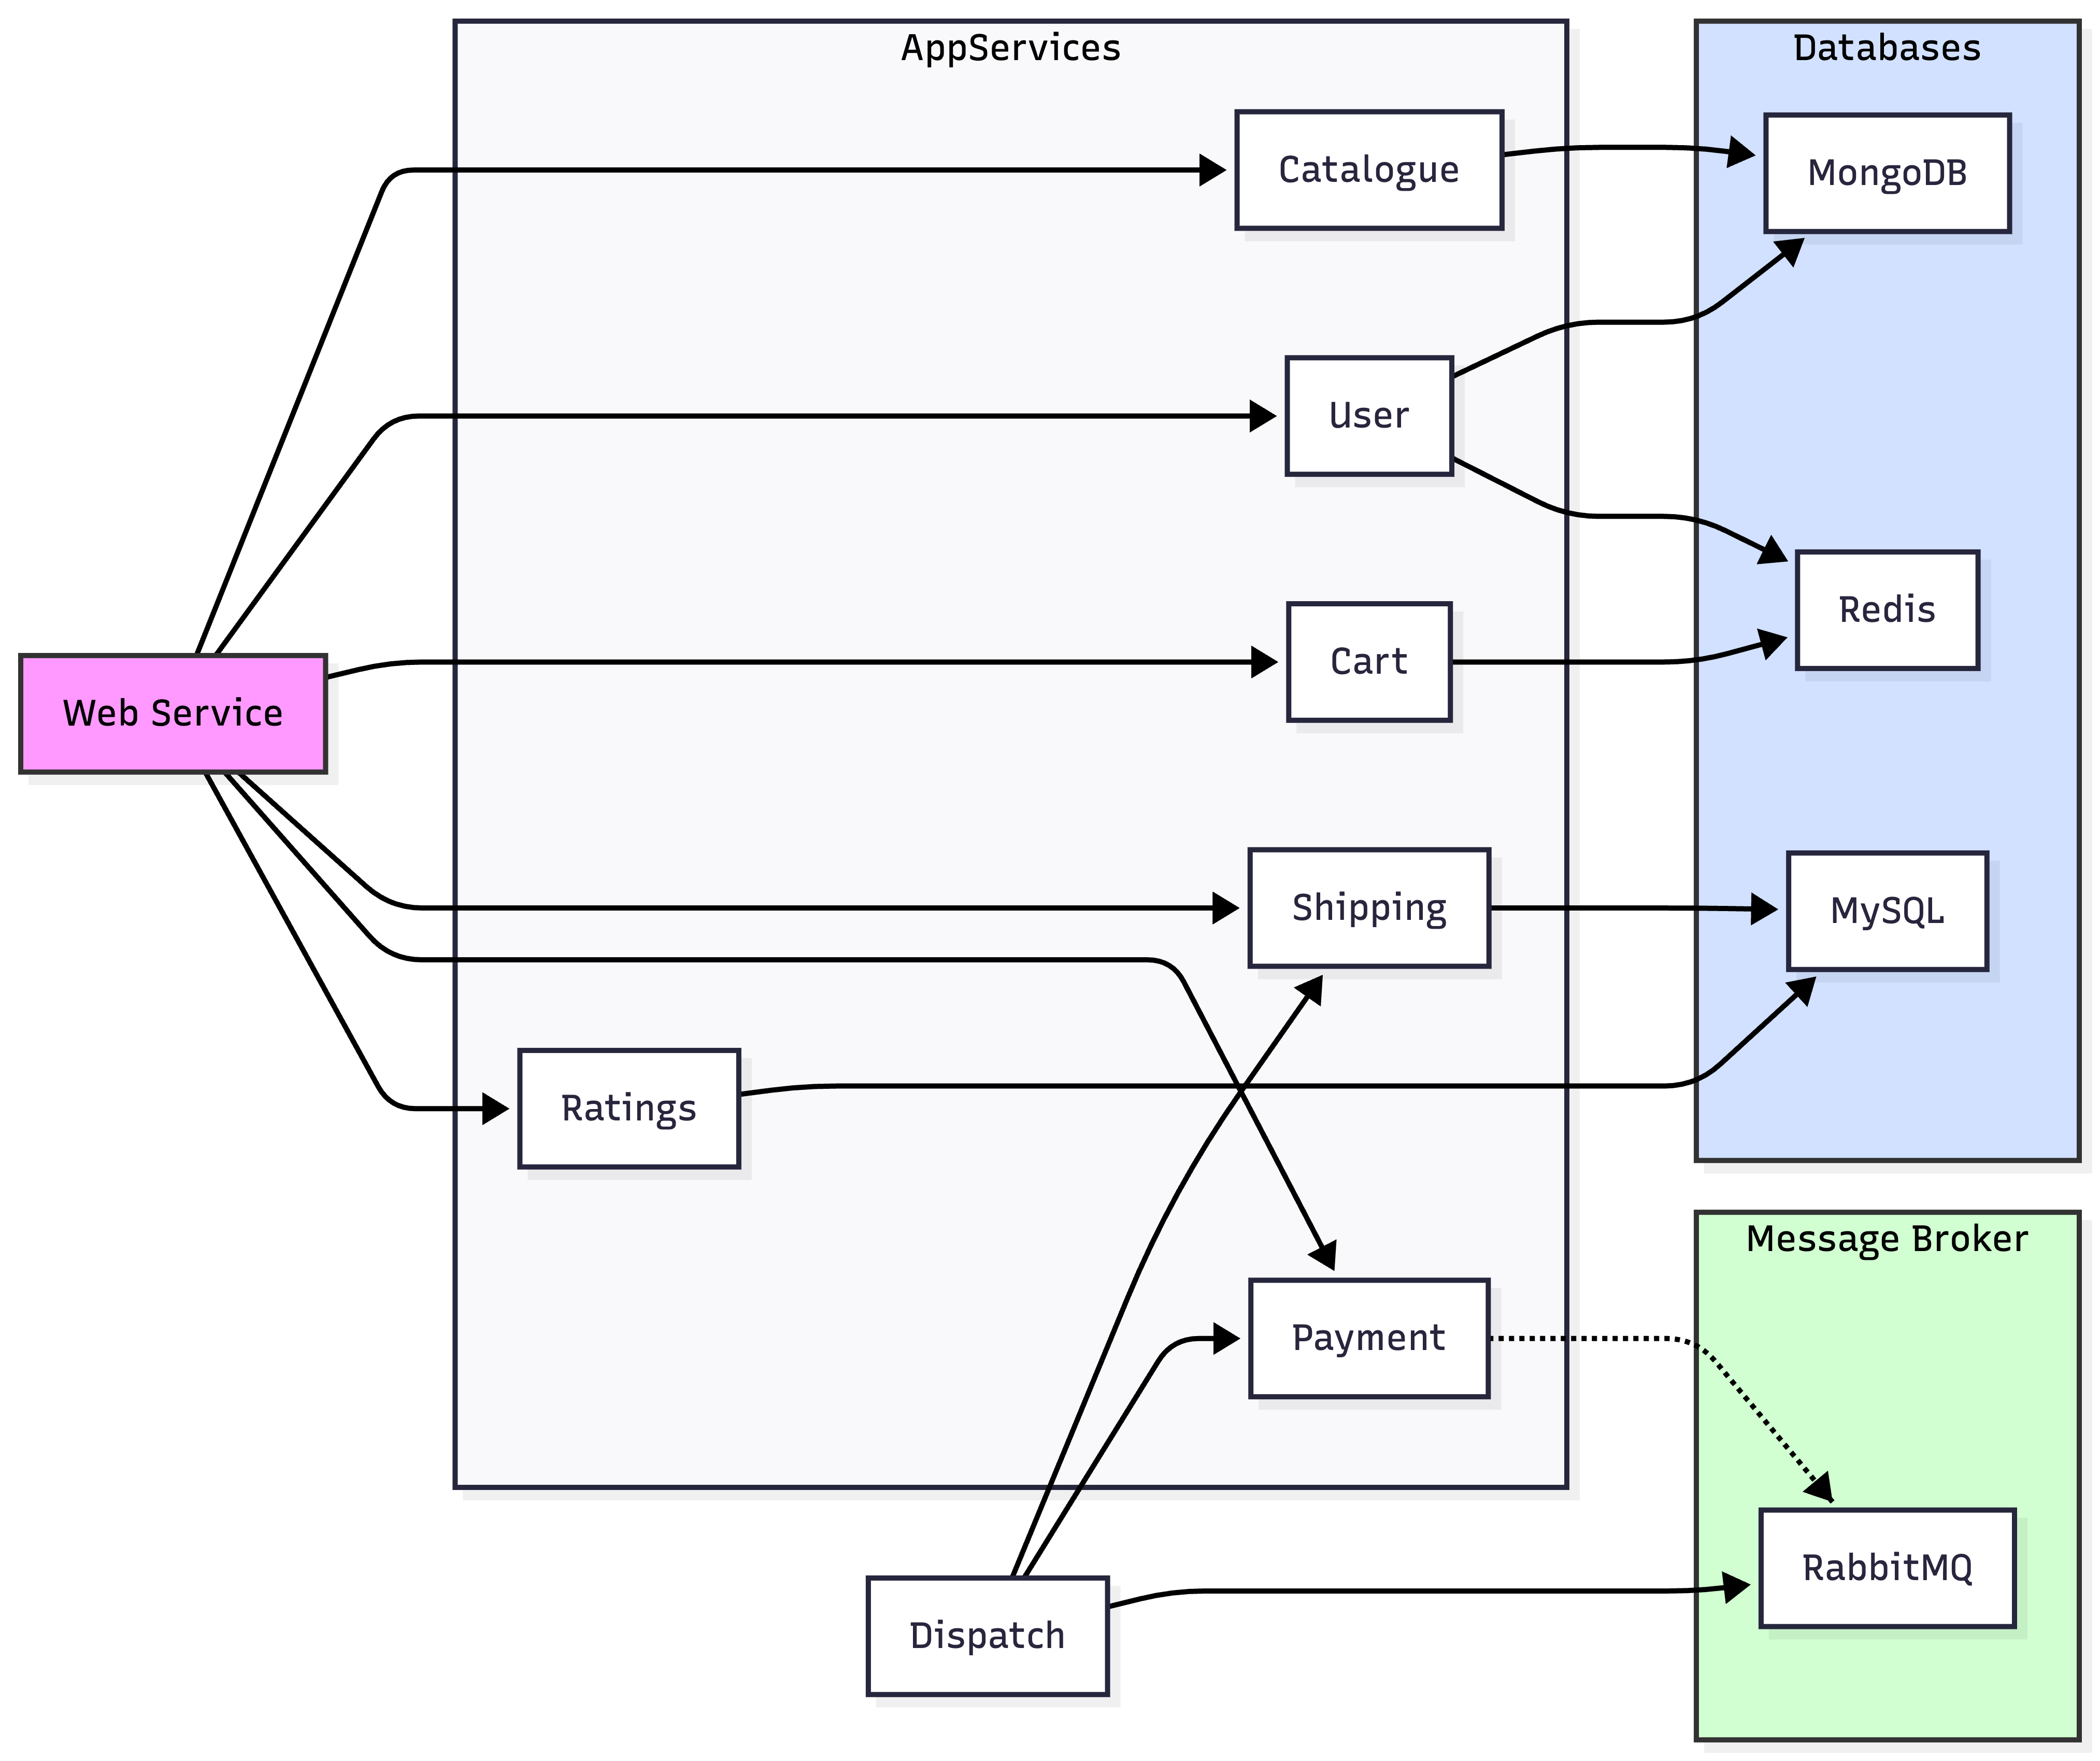
\includegraphics[width=\textwidth]{grafika/robot-shop.png}
  \caption{Architektura aplikacji Robot Shop: mikrousługi, bazy danych (MongoDB, Redis, MySQL) oraz broker wiadomości (RabbitMQ) do komunikacji asynchronicznej.}
  \label{fig:robot-shop-architektura}
\end{figure}

\subsection{Zasady działania aplikacji}
System składa się z następujących kluczowych komponentów:
\begin{itemize}
    \item \textbf{Web}: Frontend aplikacji serwujący interfejs użytkownika oraz pełniący rolę bramy (gateway) dla ruchu zewnętrznego.
    \item \textbf{Catalogue}: Zarządza katalogiem produktów i stanami magazynowymi, korzystając z bazy danych MongoDB.
    \item \textbf{User}: Odpowiada za autentykację i zarządzanie profilami użytkowników (MongoDB oraz Redis dla sesji).
    \item \textbf{Cart}: Obsługuje funkcjonalność koszyka zakupowego, przechowując dane w pamięci podręcznej Redis.
    \item \textbf{Shipping}: Zarządza procesami wysyłki i logistyki, wykorzystując bazę danych MySQL.
    \item \textbf{Payment}: Procesuje płatności oraz integruje się z zewnętrznymi systemami (symulowanymi), komunikując się asynchronicznie przez RabbitMQ.
    \item \textbf{Ratings}: System ocen i opinii o produktach, oparty na MySQL.
    \item \textbf{Dispatch}: Koordynuje realizację zamówień, korzystając z komunikatów w brokerze RabbitMQ.
\end{itemize}

Komunikacja między usługami odbywa się dwutorowo: synchronicznie poprzez REST API (np. Web $\rightarrow$ Catalogue) oraz asynchronicznie za pośrednictwem brokera wiadomości RabbitMQ (np. Payment $\rightarrow$ Dispatch).

\subsection{Wady architektury aplikacji}
Mimo zastosowania dobrych praktyk, architektura \textit{Robot Shop} posiada cechy, które sprzyjają występowaniu incydentów:
\begin{itemize}
    \item \textbf{Złożony graf zależności}: Wysoki stopień powiązania usług (np. usługa \textit{Web} zależy od niemal wszystkich pozostałych) zwiększa ryzyko wystąpienia kaskadowych awarii (\textit{cascading failures}).
    \item \textbf{Różnorodność systemów składowania danych}: Konieczność utrzymania MongoDB, MySQL i Redis wprowadza dodatkową złożoność operacyjną i potencjalne punkty awarii.
    \item \textbf{Brak mechanizmów izolacji (\textit{Bulkheads})}: W podstawowej konfiguracji awaria jednej usługi (np. \textit{Ratings}) może spowolnić działanie całego frontendu.
    \item \textbf{Wąskie gardła w komunikacji asynchronicznej}: Przeciążenie brokera RabbitMQ może prowadzić do opóźnień w kluczowych procesach biznesowych (np. wysyłce towaru).
\end{itemize}

\subsection{Wdrożenie aplikacji}
Aplikacja została wdrożona w chmurze AWS z wykorzystaniem usługi \textit{Amazon Elastic Kubernetes Service (EKS)}. Infrastruktura obejmuje:
\begin{itemize}
    \item \textbf{Kubernetes}: Zarządza cyklem życia kontenerów, skalowaniem i dostępnością.
    \item \textbf{Linkerd (Service Mesh)}: Zapewnia widoczność ruchu sieciowego, automatyczne szyfrowanie mTLS oraz zaawansowane mechanizmy monitoringu wydajności (L7 metrics).
    \item \textbf{Load Generator}: Dedykowany komponent symulujący ruch użytkowników, co jest niezbędne do testowania systemu pod obciążeniem i obserwacji skutków wprowadzanych anomalii.
\end{itemize}

\section{Obserwowalność}
Kluczowym elementem środowiska jest stos technologiczny \textit{Observability}, który pozwala agentom autoremediacyjnym na analizę stanu systemu:
\begin{itemize}
    \item \textbf{Prometheus \& Grafana}: Zbieranie i wizualizacja metryk systemowych (CPU, RAM) oraz aplikacyjnych (opóźnienia, liczba błędów).
    \textbf{Loki}: Centralizacja logów ze wszystkich mikrousług, umożliwiająca analizę przyczyn źródłowych.
    \item \textbf{Linkerd Viz}: Dostarcza szczegółowych informacji o topologii ruchu i stanie komunikacji między mikrousługami "z pudełka", bez modyfikacji kodu aplikacji.
\end{itemize}

\section{Generacja Incydentów}
W celu przetestowania zdolności autoremediacyjnych agentów, zaimplementowano system automatycznego wstrzykiwania usterek -- \textit{Saboteur Agent}. Jego zadaniem jest generowanie tzw. "Złotych Sabotaży" (\textit{Golden Sabotages}), czyli subtelnych błędów, które przechodzą przez standardowe testy CI/CD, ale wywołują incydenty w środowisku produkcyjnym pod obciążeniem.

\subsection{Implementacja \textit{Saboteur Agent}}
Agent oparty jest na modelu językowym \textit{Claude 3.5 Sonnet}. Proces sabotażu polega na:
\begin{enumerate}
    \item Analizie kodu źródłowego lub konfiguracji wybranej usługi.
    \item Dobraniu odpowiedniej strategii złośliwej zmiany.
    \item Wygenerowaniu poprawki (\textit{patch}), która jest syntaktycznie poprawna, ale logicznie wadliwa.
    \item Automatycznym wdrożeniu zmiany w systemie kontroli wersji i środowisku uruchomieniowym.
\end{enumerate}

\subsection{Klasy incydentów}
Incydenty podzielono na cztery klasy o wzrastającym poziomie trudności detekcji i naprawy:
\begin{itemize}
    \item \textbf{Klasa 1: Infrastruktura (Chaos)}: Symulowane przy użyciu \textit{Chaos Mesh}. Obejmuje awarie podów, opóźnienia sieciowe, utratę pakietów oraz sztuczne obciążenie zasobów (CPU/Memory).
    \item \textbf{Klasa 2: Regresje logiczne i wydajnościowe}: Wprowadzanie nieoptymalnych algorytmów, np. pętli $O(n^2)$ w krytycznych ścieżkach kodu lub zbędnych operacji na bazie danych (N+1 queries).
    \item \textbf{Klasa 3: Konfiguracja Kubernetes}: Błędne limity zasobów (wywołujące \textit{OOMKill}), sabotowanie sond gotowości (\textit{readiness probes}) czy literówki w zmiennych środowiskowych.
    \item \textbf{Klasa 4: Wycieki zasobów i stan aplikacji}: Wycieki pamięci, niepozamykane połączenia z bazą danych (\textit{connection leaks}), zakleszczenia (\textit{deadlocks}) oraz wyczerpanie puli wątków.
\end{itemize}

\subsection{Uruchomianie epizodów}
Badania prowadzone są w formie "epizodów". Każdy epizod składa się z:
\begin{enumerate}
    \item \textbf{Baseline}: Pomiar parametrów poprawnie działającego systemu.
    \item \textbf{Sabotage}: Wstrzyknięcie usterki przez \textit{Saboteur Agent}.
    \item \textbf{Remediation}: Faza działania agenta SRE, który musi zidentyfikować problem i zaproponować naprawę.
    \item \textbf{Evaluation}: Ocena skuteczności, czasu naprawy oraz poprawności wyciągniętych wniosków (post-mortem). Przeprowadzona automatycznie przy pomocy modelu językowego.
\end{enumerate}
\begin{figure}[H]
  \centering
  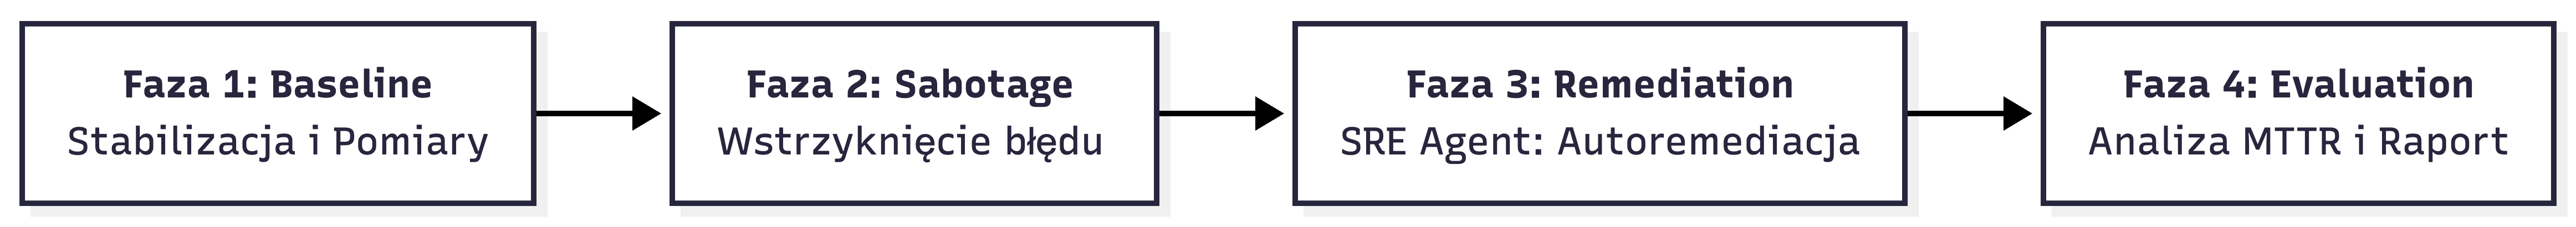
\includegraphics[width=\textwidth]{grafika/przebieg-epizodu.png}
  \caption{Przebieg faz eksperymentu dla jednego epizodu}
  \label{fig:robot-shop-architektura}
\end{figure}
\subsection{Metryki wydajnościowe i ocena auto-remediacji}
Skuteczność fazy remediacji jest mierzona zarówno w wymiarze czasu, jak i w postaci binarnych kryteriów jakościowych. Końcowa ocena \textbf{auto-remediacji} jest wykonywana \textbf{automatycznie} przez dedykowanego agenta-sędziego opartego na modelu językowym, po zakończeniu (lub przekroczeniu limitu czasu) działania agenta SRE.

\paragraph{Potok oceny (implementacja eksperymentalna).}
Po zakończeniu próby naprawy program:
\begin{enumerate}
    \item odczekuje ustalony czas stabilizacji systemu po interwencji agenta SRE;
    \item ponownie zbiera z agregatora metryk (\textit{Grafana}) zestawienie stanu klastra i usług w oknie czasowym;
    \item porównuje bieżące metryki z metrykami z fazy po sabotażu (wykrycie różnic, raport odzyskania --- m.in.\ obciążenie CPU, pamięć, kody odpowiedzi HTTP);
    \item buduje raport \textit{System Execution Evidence}: faktycznie wywołane narzędzia (w szczególności czy wywołano wdrożenie aplikacji) oraz lista zmodyfikowanych plików --- tak, by ocena nie opierała się wyłącznie na deklaracjach agenta w konwersacji;
    \item przekazuje \textit{sędziemu}: Raport \textit{Post-mortem}, raport różnic metryk oraz powyższy dowód wykonania \textit{System Execution Evidence}.
\end{enumerate}
\textit{Sędzia} ocenia wynik wyłącznie na podstawie tych materiałów; jeśli agent twierdzi, że wdrożył zmianę, a w dowodzie wykonania brak odpowiedniego wywołania narzędzia, uznaje się, że czynność nie została wykonana.

\paragraph{Wskaźniki.}
\begin{enumerate}
    \item \textbf{Time-to-Resolution (TTR)}: czas ścienny od rozpoczęcia działania agenta SRE do zakończenia próby remediacji (w eksperymencie ograniczony maksymalnym czasem oczekiwania na odpowiedź agenta), wyrażony w sekundach.
    \item \textbf{Poprawna diagnoza}: wartość 0 lub 1 --- czy agent prawidłowo wskazał faktyczną przyczynę incydentu (np.\ konkretny fragment kodu lub błędny parametr konfiguracji), zgodnie z usterką w scenariuszu.
    \item \textbf{Skuteczna naprawa}: wartość 0 lub 1 --- czy zastosowano poprawkę we właściwym miejscu (nieidentyczna z kodem sprzed incydentu, gdy dotyczy plików) \textbf{oraz} czy faktycznie uruchomiono wdrożenie (weryfikowane w dowodzie wykonania); bez potwierdzonego wdrożenia kryterium jest niespełnione.
    \item \textbf{Widoczna regeneracja w metrykach} (\texttt{system\_recovery\_visible}): wartość 0 lub 1 --- czy raport metryk po próbie naprawy wskazuje powrót do stanu zdrowego; m.in.\ obecność odpowiedzi 5xx w metrykach lub obniżenie kluczowych wskaźników względem stanu po incydencie skutkuje oceną negatywną (zgodnie z kryteriami sędziego).
\end{enumerate}